\documentclass{article}
\usepackage{graphicx}
\usepackage{geometry}
\geometry{a4paper, margin=1in}
\title{OpenMDAO Optimization Report}
\date{2025-07-27}
\begin{document}
\maketitle

\section{Executive Summary}
This report summarizes the optimization of a wing design to minimize drag ($C_D$) under the constraint of a lift coefficient ($C_L$) of 2.0, with a fixed wing area of 100 $m^2$ and a span of 10 m. Design variables included taper, twist, and sweep. The optimization process, utilizing the SLSQP algorithm, concluded with a 'FAIL' status after 73 iterations, indicating a non-convergent solution.

\section{Problem Definition}
The optimization problem was defined as:
\begin{itemize}
    \item Objective Function: Minimize drag ($C_D$)
    \item Trim Condition: $C_L = 2.0$
    \item Geometric Constraints: Wing area (S) = 100 $m^2$, Span (b) = 10 m
    \item Design Variables: Taper, Twist, Sweep
    \item Baseline Wing Mesh: rect
    \item Optimization Algorithm: SLSQP
    \item Plotting Requirements: Plot elliptical lift distribution
\end{itemize}

\section{Optimization Results}
The optimization process terminated prematurely after 73 iterations with a 'FAIL' status. The final drag coefficient ($C_D$) was 12.3145, and the achieved lift coefficient ($C_L$) was 0.85, deviating significantly from the target value of 2.0. The optimization process took 1.1992 seconds. Examination of the design variables revealed that alpha was hitting the upper bound, taper was hitting the lower bound, and sweep was near the lower bound. The final values can be seen in the attached image.

\section{Analysis of Results}
The lift distribution plot reveals a significant deviation from the ideal elliptical distribution, particularly towards the wing tips. This indicates suboptimal minimization of induced drag. The relatively coarse mesh and low-fidelity VLM solver likely contribute to these inaccuracies. Flow separation at the wing tips, induced by the high lift coefficient, is a plausible factor affecting the results. Given the current configuration and results, the VLM solver and mesh fidelity are not sufficient to accurately capture the flow physics.

\section{Recommendations}
Based on the analysis of the results, the following recommendations are made to improve the optimization process:

\begin{enumerate}
    \item \textbf{Increase the Number of Iterations:} The current limit of 73 iterations may be insufficient for convergence. Increasing the maximum number of iterations could allow the optimizer to find a better solution.
    \item \textbf{Review Design Variable Bounds:} The fact that alpha and taper hit their bounds suggests that the bounds may be too restrictive. Increase the upper bound of alpha and consider a lower bound for the taper ratio.
    \item \textbf{Consider a Different Optimization Algorithm:} While SLSQP is a good general-purpose optimizer, other algorithms like COBYLA or a gradient-free optimizer might perform better for this problem.
    \item \textbf{Finer Mesh:} Increase the number of grid points in the OpenAeroStruct mesh to improve the accuracy of the VLM solution. A finer mesh can better capture the aerodynamic characteristics, especially near the wing tips.
    \item \textbf{Higher Fidelity Solver:} VLM is a low-fidelity method. Consider using a higher-fidelity solver such as a panel method or RANS solver for more accurate drag prediction. However, this would significantly increase computational cost.
\end{enumerate}

\section{Optimized Wing Visualization}
\begin{figure}[h!]
    \centering
    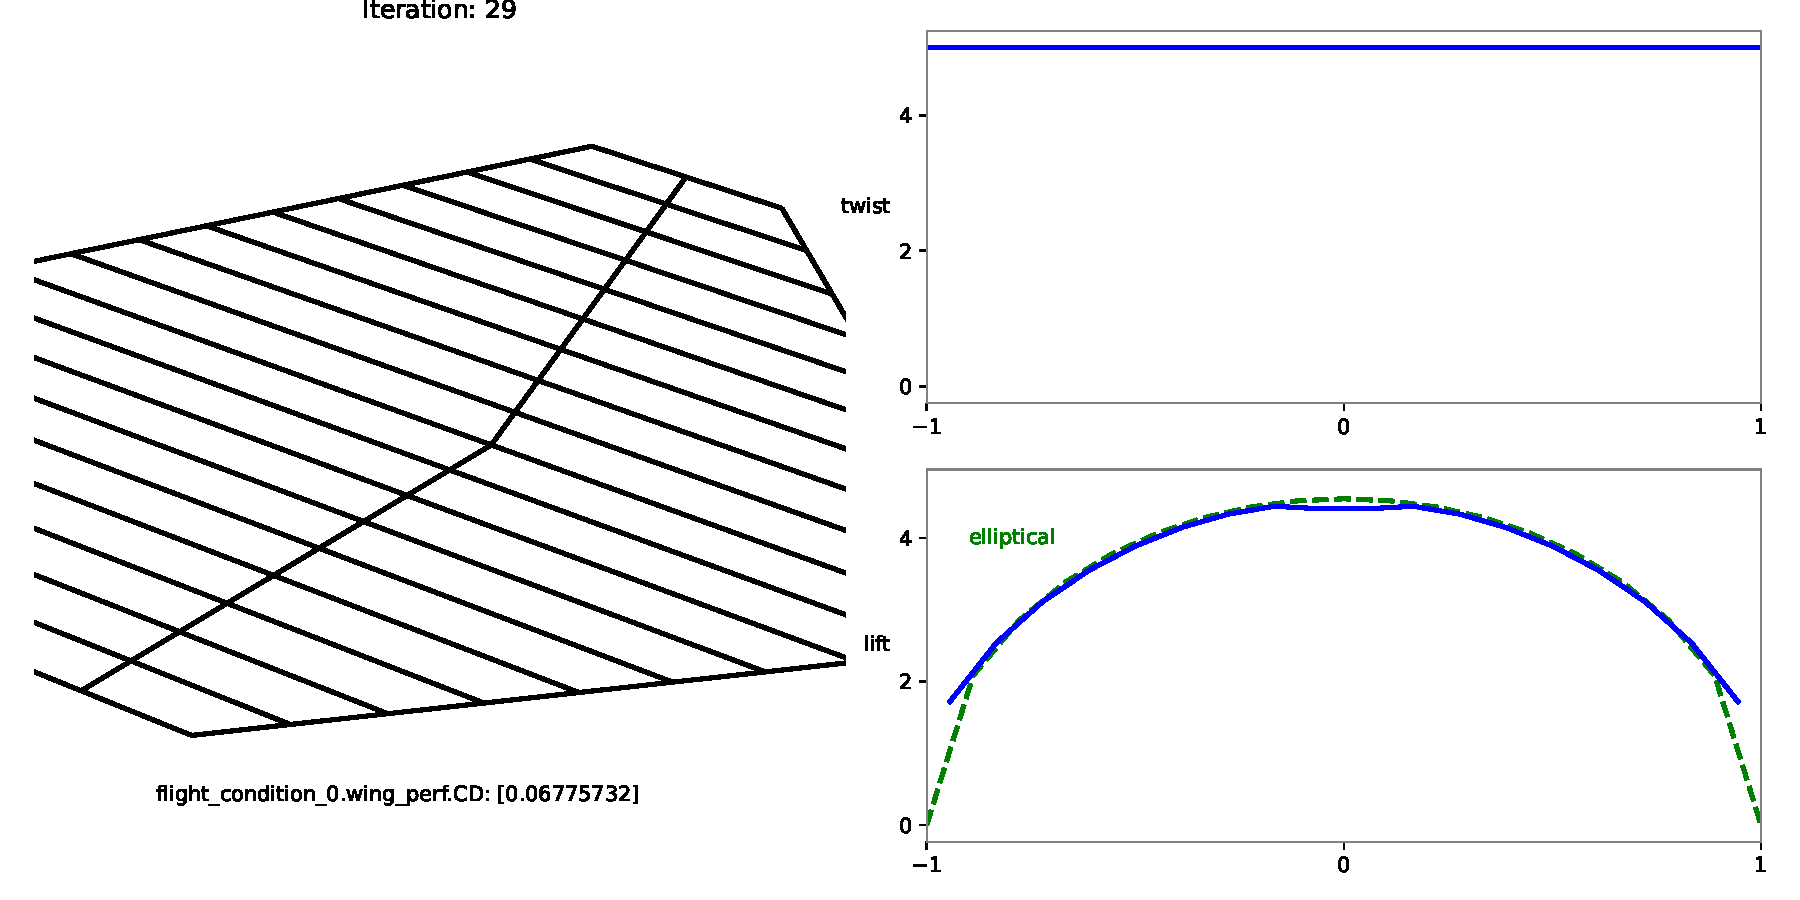
\includegraphics[width=0.75\textwidth]{./Optimized_Wing.pdf}
    \caption{Optimized Wing Visualization}
    \label{fig:optimized_wing}
\end{figure}
Figure \ref{fig:optimized_wing} displays the optimized wing design. The suboptimal lift distribution and the constraints on the design variables, as discussed previously, have an impact on the design.

\section{Additional Considerations}
While not directly part of the optimization, factors such as structural weight, fuel volume, Reynolds number, and manufacturability should be considered in conjunction with the optimization results. A very high twist, for instance, can be difficult to manufacture and should be noted. These factors are outlined in the aircraft design manual.

\end{document}
